\documentclass{article}
\usepackage[utf8]{inputenc}
% are all of these packages really necessary?
% no.
% i'm just too lazy to only grab the packages i want for a specific
% document, so i just glob all of my most commonly used packages together
% this is bad practice.
\usepackage{amsmath,amsthm,amssymb,amsfonts, fancyhdr, color, comment, graphicx, environ, mdframed, soul, calc, enumitem, mdframed, xcolor, geometry, empheq, mathtools, tikz, pgfplots, caption, subcaption, hyperref}

\usetikzlibrary{external}
\tikzexternalize[prefix=tikz/,optimize command away=\includepdf]

%tikzpicture
\usepackage{tikz}
\usepackage{scalerel}
\usepackage{pict2e}
\usepackage{tkz-euclide}
\usetikzlibrary{calc}
\usetikzlibrary{patterns,arrows.meta}
\usetikzlibrary{shadows}
\usetikzlibrary{external}

%pgfplots
\usepackage{pgfplots}
\pgfplotsset{compat=newest}
\usepgfplotslibrary{statistics}
\usepgfplotslibrary{fillbetween}
\usepgfplotslibrary{polar}

\tikzset{external/export=true}
\pgfplotsset{
    standard/.style={
    axis line style = thick,
    trig format=rad,
    enlargelimits,
    axis x line=middle,
    axis y line=middle,
    enlarge x limits=0.15,
    enlarge y limits=0.15,
    every axis x label/.style={at={(current axis.right of origin)},anchor=north west},
    every axis y label/.style={at={(current axis.above origin)},anchor=south east}
    }
}
\newcommand*\widefbox[1]{\fbox{\hspace{2em}#1\hspace{2em}}}
% Command "alignedbox{}{}" for a box within an align environment
% Source: http://www.latex-community.org/forum/viewtopic.php?f=46&t=8144
\newlength\dlf  % Define a new measure, dlf
\newcommand\alignedbox[2]{
% Argument #1 = before & if there were no box (lhs)
% Argument #2 = after & if there were no box (rhs)
&  % Alignment sign of the line
{
\settowidth\dlf{$\displaystyle #1$}  
    % The width of \dlf is the width of the lhs, with a displaystyle font
\addtolength\dlf{\fboxsep+\fboxrule}  
    % Add to it the distance to the box, and the width of the line of the box
\hspace{-\dlf}  
    % Move everything dlf units to the left, so that & #1 #2 is aligned under #1 & #2
\boxed{#1 #2}
    % Put a box around lhs and rhs
}
}

\hypersetup{
    colorlinks=true,
    linkcolor=blue,
    filecolor=magenta,      
    urlcolor=cyan,
    pdftitle={Midterm 1 Review Solutions},
    pdfpagemode=UseOutlines,
    bookmarksopen=true,
    pdfauthor={Christina Phan}
}
\newcommand{\lrp}[1]{\left( #1 \right)}
\newcommand{\abs}[1]{\left\vert #1 \right\vert}
\newcommand{\lra}[1]{\left\langle #1 \right\rangle}
\newcommand{\lrb}[1]{\left[ #1 \right]}
\newcommand{\iintR}[0]{\iint\limits_{R}}

\geometry{letterpaper, portrait, margin=1in}
\renewcommand{\footrulewidth}{0.8pt}
\setlength\parindent{0pt}
\pagestyle{fancy}
\lhead{Christina Phan}
\rhead{MAT 21D} 
\chead{\textbf{Midterm 1 Review Solutions}}

\newcommand{\Solution}{\textit{Solution}}
\pgfplotsset{compat=1.18}
\begin{document}
\phantomsection
\addcontentsline{toc}{section}{Problem 1 (Parts)}\textbf{Problem 1 (Parts)}

Evaluate the integral:

\phantomsection
\addcontentsline{toc}{subsection}{1(a)}\textbf{(a)} $\displaystyle \int_0^1\int_0^{x^3}e^{y/x}\,dy\,dx$

\Solution
\begin{align*}
    \int_0^1\int_0^{x^3}e^{y/x}\,dy\,dx&=\int_0^1 \lrb{xe^{y/x}}_0^{x^3}\,dx\\
    &=\int_0^1 xe^{x^2} - xe^{0/x}\,dx\\
    &=\int_0^1 xe^{x^2}-x\,dx\tag{$e^0=1$}\\
    &=\lrb{\frac{1}{2}e^{x^2}-\frac{1}{2}x^2}_0^1\\
    &=\lrp{\frac{1}{2}e-\frac{1}{2}}-\lrp{\frac{1}{2}e^0-0}\\
    &=\boxed{\frac{1}{2}e-1}
\end{align*}
\addcontentsline{toc}{subsection}{1(b)}\textbf{(b)} $\displaystyle\int_0^1\int_{\sqrt{y}}^{2-\sqrt{y}}xy\,dx\,dy$

\Solution

\begin{align*}
    \int_0^1\int_{\sqrt{y}}^{2-\sqrt{y}}xy\,dx\,dy &=\int_0^1 \lrb{\frac{1}{2}x^2y}_{\sqrt{y}}^{2-\sqrt{y}}\,dy\\
    &=\int_0^1\lrp{\frac{1}{2}\lrp{2-\sqrt{y}}^2y}-\lrp{\frac{1}{2}(y)y}\,dy\\
    &=\int_0^1 \lrp{\frac{1}{2}\lrp{4-4\sqrt{y}+y}y}-\frac{1}{2}y^2\,dy\\
    &=\int_0^1 2 y- 2y^{3/2}+\frac{1}{2}y^2 -\frac{1}{2}y^2\,dy\\
    &=\int_0^1 2 y- 2y^{3/2}\,dy\\
    &=\lrb{y^2-\frac{4}{5}y^{5/2}}_0^1\\
    &=\boxed{\frac{1}{5}}
\end{align*}
\phantomsection
\addcontentsline{toc}{subsection}{1(c)}\textbf{(c)} $\displaystyle \int_0^2\int_{y/2}^1 e^{x^2}\,dx\,dy$

\Solution

It might be a good idea to change our order of integration, so let's graph the region and see how we can reverse the order of integration. Let's graph $y=0$, $y=2$, $x=\dfrac{y}{2}$, and $x=1$.
\begin{center}
\resizebox{3cm}{!}{
    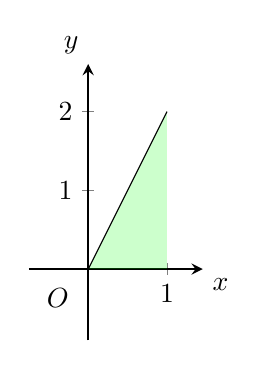
\begin{tikzpicture}
    \begin{axis}[standard,
            xtick={1},
            ytick={1,2},
            samples=1000,
            xlabel={$x$},
            ylabel={$y$},
            xmin=-0.5,xmax=1.2,
            ymin=-0.5,ymax=2.2,
            x=1cm,
            y=1cm/1
           ]
\node[anchor=center,label=south west:$O$] at (axis cs:0,0){};
\addplot[name path=F,domain={0:1}]{2*x};
\addplot[name path=G,domain={0:1}]{0};
\addplot[fill=green, fill opacity=0.2] fill between [of=F and G,soft clip={domain=0:1}];
    \end{axis}
    \end{tikzpicture}
}
\end{center}
In terms of $x$, our lower and upper bounds for $y$ are $y=0$ and $y=2x$ (from $x=y/2$), respectively.

Our lower and upper bounds for $x$ are $x=0$ and $x=1$, respectively.

Putting this all together, we get
\begin{align*}
    \int_0^2\int_{y/2}^1 e^{x^2}\,dx\,dy&=\int_0^1\int_{0}^{2x} e^{x^2}\,dy\,dx\\
    &=\int_0^1 \lrb{e^{x^2}y}_{0}^{2x}\,dx\\
    &=\int_0^1 2xe^{x^2}\,dx\\
    &=\lrb{e^{x^2}}_0^1\\
    &=\boxed{e-1}
\end{align*}
\phantomsection
\addcontentsline{toc}{subsection}{1(d)}\textbf{(d)} $\displaystyle \int_0^1\int_{\sqrt[3]{y}}^1\frac{2\pi\sin\pi x^2}{x^2}\,dx\,dy$

\Solution

It might be a good idea to change our order of integration, so let's graph the region and see how we can reverse the order of integration. Let's graph $y=0$, $y=1$, $x=\sqrt[3]{y}$, and $x=1$.

\begin{center}
\resizebox{3cm}{!}{
    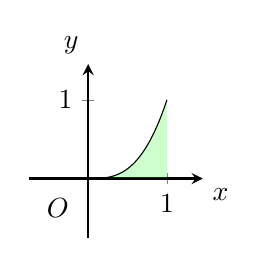
\begin{tikzpicture}
    \begin{axis}[standard,
            xtick={1},
            ytick={1},
            samples=1000,
            xlabel={$x$},
            ylabel={$y$},
            xmin=-0.5,xmax=1.2,
            ymin=-0.5,ymax=1.2,
            x=1cm,
            y=1cm/1
           ]
\node[anchor=center,label=south west:$O$] at (axis cs:0,0){};
\addplot[name path=F,domain={0:1}]{x^3};
\addplot[name path=G,domain={0:1}]{0};
\addplot[fill=green, fill opacity=0.2] fill between [of=F and G,soft clip={domain=0:1}];
    \end{axis}
    \end{tikzpicture}
}
\end{center}
In terms of $x$, our lower and upper bounds for $y$ are $y=0$ and $y=x^3$ (from $x=\sqrt[3]{y}$), respectively.

Our lower and upper bounds for $x$ are $x=0$ and $x=1$, respectively.

Putting this all together, we get
\begin{align*}
    \int_0^1\int_{\sqrt[3]{y}}^1\frac{2\pi\sin\pi x^2}{x^2}\,dx\,dy&=\int_0^1\int_0^{x^3}\frac{2\pi\sin\pi x^2}{x^2}\,dy\,dx\\
    &=\int_0^1\lrb{\frac{2\pi\sin\pi x^2}{x^2}y}_0^{x^3}\,dx\\
    &=\int_0^1 \lrp{\frac{2\pi\sin\pi x^2}{x^2}}x^3-0\,dx\\
    &=\int_0^1 2\pi x\sin\pi x^2\,dx\\
    &u=\pi x^2\hspace{2em} du=2\pi x\,dx\\
    &u(0)=0\hspace{2em} u(1)=\pi\\
    &=\int_0^{\pi} \sin u\,du\\
    &=\lrb{-\cos u}_0^{\pi}\\
    &= (1) - (-1)\\
    &=\boxed{2}
\end{align*}
\phantomsection
\addcontentsline{toc}{subsection}{1(e)}
\textbf{(e)} $\displaystyle \int_{-1}^1\int_{-\sqrt{1-y^2}}^{\sqrt{1-y^2}}\ln (x^2+y^2+1)\,dx\,dy$

\Solution

This looks like a great candidate for polar coordinates!

Let's graph the region to see. That is, graph $y=-1$, $y=1$, $x=-\sqrt{1-y^2}$, and $x-\sqrt{1-y^2}$.
\begin{center}
\resizebox{3cm}{!}{
    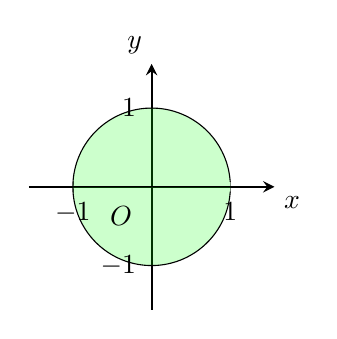
\begin{tikzpicture}
    \begin{axis}[standard,
            xtick={-1,1},
            ytick={-1,1},
            samples=1000,
            xlabel={$x$},
            ylabel={$y$},
            xmin=-1.2,xmax=1.2,
            ymin=-1.2,ymax=1.2,
            x=1cm,
            y=1cm/1
           ]
\node[anchor=center,label=south west:$O$] at (axis cs:0,0){};
\addplot[name path=F,domain={-1:1}]{sqrt(1-x^2)};
\addplot[name path=G,domain={-1:1}]{-sqrt(1-x^2)};
\addplot[name path=H,domain={-1:1}]{0};
\addplot[fill=green, fill opacity=0.2] fill between [of=F and H,soft clip={domain=-1:1}];
\addplot[fill=green, fill opacity=0.2] fill between [of=G and H,soft clip={domain=-1:1}];
    \end{axis}
    \end{tikzpicture}
}
\end{center}

Our lower and upper bounds for $r$ are $r=0$ and $r=1$, respectively.

Our lower and upper bounds for $\theta$ are $\theta=0$ and $\theta =2\pi$, respectively.

Putting this all together, we get
\begin{align*}
    \int_{-1}^1\int_{-\sqrt{1-y^2}}^{\sqrt{1-y^2}}\ln (x^2+y^2+1)\,dx\,dy&=\int_0^{2\pi}\int_0^1 \big(\ln (r^2+1)\big)r\,dr\,d\theta\tag{don't forget extra $r$; $x^2+y^2=r^2$}\\
    &u=r^2 +1\hspace{2em} du=2r\,dr\\
    &u(0)=1\hspace{2em} u(1) = 2\\
    &=\int_0^{2\pi}\frac{1}{2}\int_1^2 \ln u\,du\,d\theta\\
    &v=\ln u\hspace{2em}dw=\,du\\
    &dv=\frac{1}{u}\,du\hspace{2em}w=u\\
    &=\int_0^{2\pi}\frac{1}{2}\lrp{\lrb{u\ln u}_1^2-\int_1^2 \,du}\,d\theta\\
    &=\int_0^{2\pi}\frac{1}{2}\lrp{2\ln 2 - 1\ln 1 - \lrb{u}_1^2}\,d\theta\\
    &=\int_0^{2\pi}\frac{1}{2}\lrp{2\ln 2 - (2-1)}\,d\theta\\
    &=\int_0^{2\pi}\frac{1}{2}\lrp{2\ln 2-1}\,d\theta\\
    &=\int_0^{2\pi} \ln 2 -\frac{1}{2}\,d\theta\\
    &=\lrb{(\ln 2)\theta -\frac{1}{2}\theta}_0^{2\pi}\\
    &=2(\ln 2) \pi - \pi\\
    &=\boxed{(\ln 4) \pi-\pi}\tag{$2\ln 2=\ln 2^2=\ln 4$}
\end{align*}
\phantomsection
\addcontentsline{toc}{subsection}{1(f)}
\textbf{(f)} $\displaystyle \int_1^e\int_1^x\int_0^z\frac{2y}{z^3}\,dy\,dz\,dx$

\Solution
\begin{align*}
    \int_1^e\int_1^x\int_0^z\frac{2y}{z^3}\,dy\,dz\,dx&=\int_1^e\int_1^x \lrb{\frac{y^2}{z^3}}_0^z\,dz\,dx\\
    &=\int_1^e\int_1^x \frac{z^2}{z^3}-0\,dz\,dx\\
    &=\int_1^e\int_1^x \frac{1}{z}\,dz\,dx\\
    &=\int_1^e \lrb{\ln \left|z\right|}_1^x\,dx\\
    &=\int_1^e \ln x - \ln 1\,dx\tag{ok to drop abs since $1\leq x\leq e$}\\
    &=\int_1^e \ln x\,dx\\
    &u=\ln x\hspace{2em}dv=dx\\
    &du=\frac{1}{x}\,dx\hspace{2em}v=x\\
    &=\lrb{x\ln x}_1^e -\int_1^e \,dx\\
    &=\lrp{e\ln e - \ln 1}-\lrb{x}_1^e\\
    &= \lrp{e - 0}-\lrp{e-1}\\
    &=\boxed{ 1}
\end{align*}
\phantomsection
\addcontentsline{toc}{section}{Problem 2}\textbf{Problem 2} 

Find the volume under the paraboloid $z = x^2 +y^2$ above the triangle enclosed by $y = x$,
$x = 0$, and $x + y = 2$ in the $xy$-plane.

\Solution

Let's draw our region. That is, graph $y=x$, $x=0$, and $x+y=2$.
\begin{center}
\resizebox{3cm}{!}{
    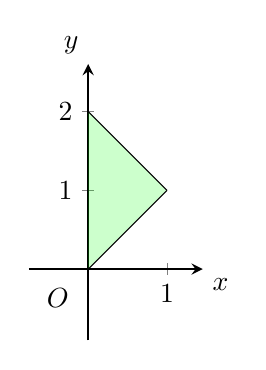
\begin{tikzpicture}
    \begin{axis}[standard,
            xtick={1},
            ytick={1,2},
            samples=1000,
            xlabel={$x$},
            ylabel={$y$},
            xmin=-0.5,xmax=1.2,
            ymin=-0.5,ymax=2.2,
            x=1cm,
            y=1cm/1
           ]
\node[anchor=center,label=south west:$O$] at (axis cs:0,0){};
\addplot[name path=F,domain={0:1}]{x};
\addplot[name path=G,domain={0:1}]{2-x};
\addplot[fill=green, fill opacity=0.2] fill between [of=F and G,soft clip={domain=0:1}];
    \end{axis}
    \end{tikzpicture}
}
\end{center}

Our lower and upper bounds for $y$ are $y=x$ and $y=-x+2$, respectively.

Our lower and upper bounds for $x$ are $x=0$ and $x=1$, respectively.

Putting this all together, we get
\begin{align*}
    V&=\int_0^1\int_{x}^{-x+2} x^2+y^2\,dy\,dx\\
    &=\int_0^1 \lrb{x^2y+\frac{1}{3}y^3}_{x}^{-x+2}\,dx\\
    &=\int_0^1 \lrp{x^2(-x+2)+\frac{1}{3}(-x+2)^3}-\lrp{x^3+\frac{1}{3}x^3}\,dx\\
    &= \int_0^1 -x^3 + 2x^2 +\frac{1}{3}(-x+2)^3 -\frac{4}{3}x^3\,dx\\
    &=\int_0^1 2x^2 -\frac{7}{3}x^3 +\frac{1}{3}(-x+2)^3\,dx\\
    &=\lrb{\frac{2}{3}x^3-\frac{7}{12}x^4-\frac{1}{12}(-x+2)^4}_0^1\\
    &=\lrp{\frac{2}{3}-\frac{7}{12}-\frac{1}{12}}-\lrp{0-0-\frac{1}{12}(2)^4}\\
    &=\boxed{\frac{4}{3}}\tag{use a calculator :)}
\end{align*}
\phantomsection
\addcontentsline{toc}{section}{Problem 3}\textbf{Problem 3}

Find the average value of the function $f(x,y) = xy$ over the quarter circle $x^2 + y^2 = 1$
in the first quadrant.

\Solution

Recall that the average value of $f(x,y)$ is
\begin{align*}
    f(x,y)_{\text{avg}}=\frac{1}{A}\iint_R f(x,y)\,dA
\end{align*}
where $A$ is the area of the region $R$.

Let's graph the region $R$. That is, graph $y=\sqrt{1-x^2}$ in the first quadrant.
\begin{center}
\resizebox{3cm}{!}{
    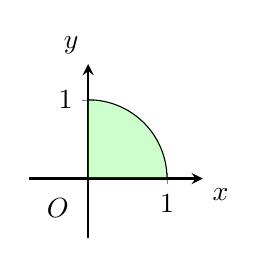
\begin{tikzpicture}
    \begin{axis}[standard,
            xtick={1},
            ytick={1},
            samples=1000,
            xlabel={$x$},
            ylabel={$y$},
            xmin=-0.5,xmax=1.2,
            ymin=-0.5,ymax=1.2,
            x=1cm,
            y=1cm/1
           ]
\node[anchor=center,label=south west:$O$] at (axis cs:0,0){};
\addplot[name path=F,domain={0:1}]{sqrt(1-x^2)};
\addplot[name path=G,domain={0:1}]{0};
\addplot[fill=green, fill opacity=0.2] fill between [of=F and G,soft clip={domain=0:1}];
    \end{axis}
    \end{tikzpicture}
}
\end{center}

The lower bound of $y$ in terms of $x$ is $y=0$ and $y=\sqrt{1-x^2}$, respectively.

The lower bound of $x$ is $x=0$ and $x=1$, respectively.
\begin{align*}
    f(x,y)_{\text{avg}}&=\frac{1}{\frac{1}{4}\pi}\int_0^1\int_{0}^{\sqrt{1-x^2}}xy\,dy\,dx\\
    &=\frac{4}{\pi}\int_0^1\lrb{\frac{1}{2}xy^2}_0^{\sqrt{1-x^2}}\,dx\\
    &=\frac{4}{\pi}\int_0^1 \frac{1}{2}x(1-x^2)\,dx\\
    &=\frac{2}{\pi}\int_0^1 x(1-x)^2\,dx\\
    &=\frac{2}{\pi}\int_0^1 x-x^3\,dx\\
    &=\frac{2}{\pi}\lrb{\frac{1}{2}x^2-\frac{1}{4}x^4}_0^1\\
    &=\frac{2}{\pi}\lrp{\frac{1}{2}-\frac{1}{4}}\\
    &=\frac{2}{\pi}\lrp{\frac{1}{4}}\\
    &=\boxed{\frac{1}{2\pi}}
\end{align*}
\phantomsection
\addcontentsline{toc}{section}{Problem 4}\textbf{Problem 4}

Find the volume of the region enclosed on the top by the plane $z = -2x$, on the side by the cylinder $x = -\cos y$, $\displaystyle -\frac{\pi}{2}\leq y\leq \frac{\pi}{2}$, and below by the $xy$-plane.

\Solution

Our lower and upper bounds for $z$ are $z=0$ (the $xy$-plane) and $z=-2x$, respectively.

Our lower and upper bounds for $x$ in terms of $y$ are $x=-\cos y$ and $x=0$ ($z=-2x\implies 0=-2x\implies x=0$), respectively.

Our lower and upper bounds for $y$ are $y=-\dfrac{\pi}{2}$ and $y=\dfrac{\pi}{2}$, respectively.

Putting this all together, we get
\begin{align*}
    V&=\int_{-\pi/2}^{\pi/2}\int_{-\cos y}^{0}\int_{0}^{-2x}\,dz\,dx\,dy\\
    &=\int_{-\pi/2}^{\pi/2}\int_{-\cos y}^{0}\lrb{z}_{0}^{-2x}\,dx\,dy\\
    &=\int_{-\pi/2}^{\pi/2}\int_{-\cos y}^{0} -2x\,dx\,dy\\
    &=\int_{-\pi/2}^{\pi/2}\lrb{-x^2}_{-\cos y}^{0}\,dy\\
    &=\int_{-\pi/2}^{\pi/2}\cos^2 y\,dy\\
    &=\int_{-\pi/2}^{\pi/2} \frac{1}{2}\lrp{1+\cos 2y}\,dy\\
    &=\frac{1}{2}\int_{-\pi/2}^{\pi/2} 1+\cos 2y\,dy\\
    &=-\frac{1}{2}\lrb{y+\frac{1}{2}\sin 2y}_{-\pi/2}^{\pi/2}\\
    &=-\frac{1}{2}\lrp{\lrp{\frac{\pi}{2}-0}-\lrp{-\frac{\pi}{2}-0}}\\
    &=\boxed{\frac{1}{2}\pi}
\end{align*}
\phantomsection
\addcontentsline{toc}{section}{Problem 5}\textbf{Problem 5}

Find the average value of $f(x,y,z) = 30xz\sqrt{x^2+y}$ over the rectangular solid in the
first octant bounded by the coordinate planes and the planes $x = 1$, $y = 3$, $z = 1$.

\Solution

Recall that the average value of $f(x,y,z)$ is
\begin{align*}
    f(x,y,z)_{\text{avg}}=\frac{1}{V}\iint_R f(x,y,z)\,dA
\end{align*}
where $V$ is the volume of the region $R$.

The volume $V$ of the region $R$ would be a rectangular prism with dimensions $1\times3\times 1$.

The lower and upper bounds of $z$ are $z=0$ and $z=1$, respectively.

The lower and upper bounds of $y$ are $y=0$ and $y=3$, respectively.

The lower and upper bounds of $x$ are $x=0$ and $x=1$, respectively.
\begin{align*}
    f(x,y,z)_{\text{avg}}&=\frac{1}{(1)(3)(1)}\int_0^1\int_0^3\int_0^1 30xz\sqrt{x^2+y}\,dz\,dy\,dx\\
    &=\frac{1}{3}\int_0^1\int_0^3\lrb{15xz^2\sqrt{x^2+y}}_0^1\,dy\,dx\\
    &=\frac{1}{3}\int_0^1\int_0^3 15x\sqrt{x^2+y}\,dy\,dx\\
    &=\frac{1}{3}\int_0^3\int_0^1 15x\sqrt{x^2+y}\,dx\,dy\tag{ok since $x$ and $y$ independent}\\
    &=\frac{1}{3}\int_0^3\lrb{5(x^2+y)^{3/2}}_0^1\,dy\tag{you can also do u-sub, $u=x^2+y$}\\
    &=\frac{1}{3}\int_0^3 5(1+y)^{3/2}-5y^{3/2}\,dy\\
    &=\frac{1}{3}\lrb{2(1+y)^{5/2}-2y^{5/2}}_0^3\tag{you can also break up and do $u$ sub, $u=1+y$}\\
    &=\frac{1}{3}\lrp{\lrp{2(4)^{5/2}-2(3)^{5/2}}-\lrp{2-0}}\\
    &=\frac{1}{3}\lrp{64-2(3^{5/2})-2}\\
    &=\boxed{\frac{1}{3}\lrp{62-2(3^{5/2})}}
\end{align*}
\phantomsection
\addcontentsline{toc}{section}{Problem 6}\textbf{Problem 6}

Convert $\displaystyle \int_0^{2\pi}\int_0^{\sqrt{2}}\int_r^{\sqrt{4-r^2}}3\,dzr\,dr\,d\theta$ to rectangular coordinates in the order $dz\,dx\,dy$ and to spherical coordinates. Then evaluate one of the integrals.

\Solution

\phantomsection
\addcontentsline{toc}{subsection}{Rectangular Coordinates}\textbf{Rectangular Coordinates}

We can get our lower and upper bounds for $z$ from $z=r$ and $z=\sqrt{4-r^2}$.
\begin{align*}
    z=r&\implies z=\sqrt{x^2+y^2}\\
    z=\sqrt{4-r^2}&\implies z=\sqrt{4-x^2-y^2}
\end{align*}

To find our $y$ and $x$ bounds, let's graph the polar region $\theta =0$, $\theta = 2\pi$, $r=0$, and $r=\sqrt{2}$.

\begin{center}
\resizebox{3.5cm}{!}{
    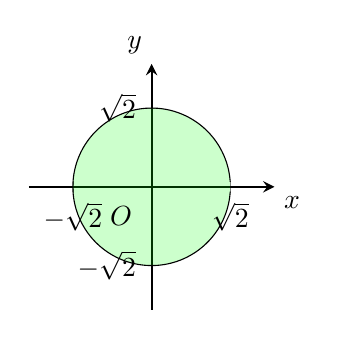
\begin{tikzpicture}
    \begin{axis}[standard,
            xtick={-1,1},
            ytick={-1,1},
            samples=1000,
            xlabel={$x$},
            ylabel={$y$},
            xmin=-1.2,xmax=1.2,
            ymin=-1.2,ymax=1.2,
            x=1cm,
            y=1cm/1,           xticklabels={$-\sqrt{2}$,$\sqrt{2}$},            yticklabels={$-\sqrt{2}$,$\sqrt{2}$}
           ]
\node[anchor=center,label=south west:$O$] at (axis cs:0,0){};
\addplot[name path=F,domain={-1:1}]{sqrt(1-x^2)};
\addplot[name path=G,domain={-1:1}]{-sqrt(1-x^2)};
\addplot[fill=green, fill opacity=0.2] fill between [of=F and G,soft clip={domain=-1:1}];
    \end{axis}
    \end{tikzpicture}
}
\end{center}
Our lower and upper bounds for $y$ in terms of $x$ are $y=-\sqrt{2-x^2}$ and $y=\sqrt{2-x^2}$, respectively.

Our lower and upper bounds for $x$ are $x=-\sqrt{2}$ and $x=\sqrt{2}$, respectively.

Putting this all together, we get
\begin{align*}
    \int_0^{2\pi}\int_0^{\sqrt{2}}\int_r^{\sqrt{4-r^2}}3\,dzr\,dr\,d\theta&=\int_{-\sqrt{2}}^{\sqrt{2}}\int_{-\sqrt{2-y^2}}^{\sqrt{2-y^2}}\int_{\sqrt{x^2+y^2}}^{\sqrt{4-x^2-y^2}}3\,dz\,dx\,dy
\end{align*}
\phantomsection
\addcontentsline{toc}{subsection}{Spherical Coordinates}\textbf{Spherical Coordinates}

We can get our lower and upper bounds for $\rho$ and $\phi$ from $z=r$ and $z=\sqrt{4-r^2}$.
\begin{align*}
    z=r&\implies \rho \cos\phi = \rho \sin \phi \implies 1 = \tan \phi \implies \phi = \frac{\pi}{4}\\
    z=\sqrt{4-r^2}&\implies z^2=4-r^2 \implies z^2+r^2 = 4\implies \rho^2 = 4\implies \rho = 2
\end{align*}
Graphically, the ``front view" looks like
\begin{center}
\resizebox{3.5cm}{!}{
    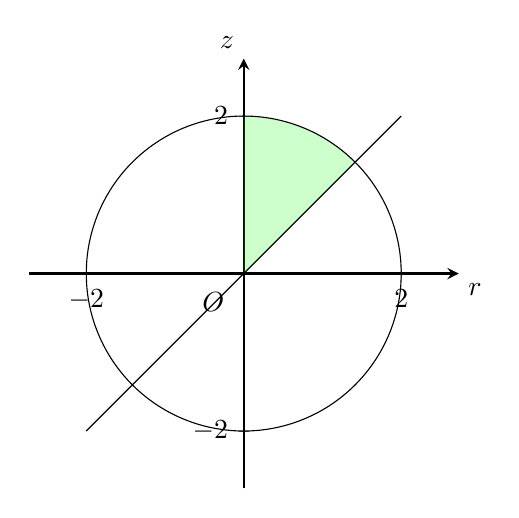
\begin{tikzpicture}
    \begin{axis}[standard,
            xtick={-2,2},
            ytick={-2,2},
            samples=1000,
            xlabel={$r$},
            ylabel={$z$},
            xmin=-2.1,xmax=2.1,
            ymin=-2.1,ymax=2.1,
            x=1cm,
            y=1cm/1,
           ]
\node[anchor=center,label=south west:$O$] at (axis cs:0,0){};
\addplot[name path=F,domain={-2:2}]{sqrt(4-x^2)};
\addplot[name path=G,domain={-2:2}]{-sqrt(4-x^2)};
\addplot[name path=H,domain={-2:2}]{x};
\addplot[fill=green, fill opacity=0.2] fill between [of=F and H,soft clip={domain=0:1.4}];
    \end{axis}
    \end{tikzpicture}
}
\end{center}
The lower and upper bounds of $\rho$ are $\rho =0$ and $\rho =2$, respectively.

The lower and upper bounds of $\phi$ are $\phi = 0$ and $\phi = \pi/4$, respectively.

We're going around the entire $z$ axis for our ``top view" so our lower and upper bounds of $\theta$ are $\theta=0$ and $\theta=2\pi$, respectively. You can check the top view from the rectangular coordinates section.

Putting this all together, we get
\begin{align*}
    \int_0^{2\pi}\int_0^{\sqrt{2}}\int_r^{\sqrt{4-r^2}}3\,dzr\,dr\,d\theta&=\int_0^{2\pi}\int_0^{\pi/4}\int_0^2 3\rho^2\sin\phi\,d\rho\,d\phi\,d\theta
\end{align*}
\phantomsection
\addcontentsline{toc}{subsection}{Evaluate Integral}\textbf{Evaluate Integral}

Based on the three integrals, cylindrical coordinate integral looks the nicest. Let's evaluate that one.
\begin{align*}
    \int_0^{2\pi}\int_0^{\sqrt{2}}\int_r^{\sqrt{4-r^2}}3\,dzr\,dr\,d\theta&=\int_0^{2\pi}\int_0^{\sqrt{2}}\lrb{3z}_r^{\sqrt{4-r^2}}\,r\,dr\,d\theta\\
    &=\int_0^{2\pi}\int_0^{\sqrt{2}} (3\sqrt{4-r^2}-3r)r\,dr\,d\theta\\
    &=\int_0^{2\pi}\int_0^{\sqrt{2}} 3r\sqrt{4-r^2}-3r^2\,dr\,d\theta\\
    &=\int_0^{2\pi} \lrb{-(4-r^2)^{3/2}-r^3}_0^{\sqrt{2}}\,d\theta\\
    &=\int_0^{2\pi} \lrp{-(4-2)^{3/2}-2^{3/2}}-\lrp{-4^{3/2}-0}\,d\theta\\
    &=\int_0^{2\pi} -2^{3/2}-2^{3/2}+4^{3/2}\,d\theta\\
    &=\int_0^{2\pi} -2(2^{3/2}) +8\,d\theta\\
    &=\int_0^{2\pi} -2^{5/2}+8\,d\theta\\
    &=\lrb{(-2^{5/2}+8)\theta}_0^{2\pi}\\
    &=(-2^{5/2}+8)(2\pi)-0\\
    &=\boxed{-2^{7/2}\pi+16\pi}
\end{align*}
\newpage
\phantomsection
\addcontentsline{toc}{section}{Problem 7}
\textbf{Problem 7}

Write the integral of $f(x,y,z)=6+4y$ over the region in the first octant bounded by the cone $z=\sqrt{x^2+y^2}$, the cylinder $x^2+y^2=1$, and the coordinate planes in all three coordinate systems and evaluate one of the integrals.

\Solution

\phantomsection
\addcontentsline{toc}{subsection}{Cartesian Coordinates}\textbf{Cartesian Coordinates}

Our lower and upper bounds for $z$ are $z=0$ and $z=\sqrt{x^2+y^2}$, respectively.

From the ``top view", we can get our lower and upper bounds for $y$ and $x$ from the cylinder $x^2+y^2=1$. On the $xy$ plane in the first quadrant (positive $xy$ only!), this cylinder looks like
\begin{center}
\resizebox{3cm}{!}{
    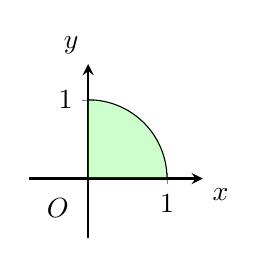
\begin{tikzpicture}
    \begin{axis}[standard,
            xtick={1},
            ytick={1},
            samples=1000,
            xlabel={$x$},
            ylabel={$y$},
            xmin=-0.5,xmax=1.2,
            ymin=-0.5,ymax=1.2,
            x=1cm,
            y=1cm/1
           ]
\node[anchor=center,label=south west:$O$] at (axis cs:0,0){};
\addplot[name path=F,domain={0:1}]{sqrt(1-x^2)};
\addplot[name path=H,domain={0:1}]{0};
\addplot[fill=green, fill opacity=0.2] fill between [of=F and H,soft clip={domain=0:1}];
    \end{axis}
    \end{tikzpicture}
}
\end{center}
Our lower and upper bounds for $y$ in terms of $x$ are $y=0$ and $y=\sqrt{1-x^2}$, respectively. Our lower bound for $y$ is not $y=-\sqrt{1-x^2}$ since we are in the first octant only.

Our lower and upper bounds for $x$ are $x=0$ and $x=1$, respectively. Our lower bound for $x$ is not $x=-1$ since we are in the first octant only.

Putting this all together, we get
\begin{align*}
    \int_{0}^1\int_{0}^{\sqrt{1-x^2}}\int_0^{\sqrt{x^2+y^2}}6+4y\,dz\,dy\,dx
\end{align*}
\addcontentsline{toc}{subsection}{Cylindrical Coordinates}\textbf{Cylindrical Coordinates}

Our lower and upper bounds for $z$ are $z=0$ and $z=\sqrt{x^2+y^2}$, respectively. In polar, our lower and upper bounds for $z$ are $z=0$ and $z=\sqrt{r^2}=r$, respectively ($x^2+y^2=r^2$).

We can get our lower and upper bounds for $r$ and $\theta$ from the ``top view". See the Cartesian Coordinate section for the graph.

Our lower and upper bounds for $r$ are $r=0$ and $r=1$ respectively (see the region in the Cartesian Coordinate section)

Our lower and upper bounds for $\theta$ are $\theta=0$ and $\theta =\dfrac{\pi}{2}$ , respectively (see the region in the Cartesian Coordinate section).

Putting this all together, we get
\begin{align*}
    \int_{0}^{\pi/2}\int_0^1\int_0^r (6+4r\sin\theta)r\,dz\,dr\,d\theta\tag{in polar, $y=r\sin\theta$}
\end{align*}
\newpage
\addcontentsline{toc}{subsection}{Spherical Coordinates}\textbf{Spherical Coordinates}

We can get our $\rho$, $\phi$, and $\theta$ bounds from looking at the front view and top view of this region. 

For the front view,  we can rewrite the cone and cylinder in terms of polar to get $z=\sqrt{r^2}=r$ and $r^2=1\implies r=1$.

For the top view, we can get the region from the cylinder $x^2+y^2=1$ in the first quadrant (positive $xy$ only!).
\begin{figure}[h]
\centering
\begin{minipage}{.5\textwidth}
  \centering
  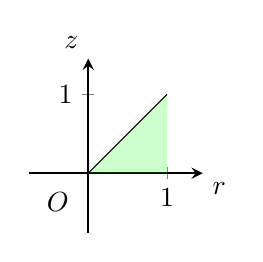
\begin{tikzpicture}
    \begin{axis}[standard,
            xtick={1},
            ytick={1},
            samples=1000,
            xlabel={$r$},
            ylabel={$z$},
            xmin=-0.5,xmax=1.2,
            ymin=-0.5,ymax=1.2,
            x=1cm,
            y=1cm/1,
           ]
\node[anchor=center,label=south west:$O$] at (axis cs:0,0){};
\addplot[name path=F,domain={0:1}]{x};
\addplot[name path=H,domain={0:1}]{0};
\addplot[fill=green, fill opacity=0.2] fill between [of=F and H, soft clip={domain=0:1}];
    \end{axis}
    \end{tikzpicture}
  \caption*{front view}
  \label{fig:test1}
\end{minipage}%
\begin{minipage}{.5\textwidth}
  \centering
  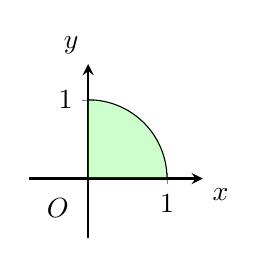
\begin{tikzpicture}
    \begin{axis}[standard,
            xtick={1},
            ytick={1},
            samples=1000,
            xlabel={$x$},
            ylabel={$y$},
            xmin=-0.5,xmax=1.2,
            ymin=-.5,ymax=1.2,
            x=1cm,
            y=1cm/1,
           ]
\node[anchor=center,label=south west:$O$] at (axis cs:0,0){};
\addplot[name path=F,domain={0:1}]{sqrt(1-x^2)};
\addplot[name path=H, domain={0:1}]{0};
\addplot[fill=green, fill opacity=0.2] fill between [of=F and H, soft clip={domain=0:1}];
    \end{axis}
    \end{tikzpicture}
  \caption*{top view}
  \label{fig:test2}
\end{minipage}
\end{figure}

Our upper bound of $\rho$ is from $r=1\implies \rho \sin\phi = 1\implies \rho =\csc\phi$.

Therefore, the lower and upper bounds of $\rho$ are $\rho = 0$ and $\rho = \csc\phi$, respectively.

We know that the lower bound of $\phi$ is $\dfrac{\pi}{4}$ because the lower bound of $\phi$ occurs when $z=r=1$ which means $\tan\phi = 1$.

Therefore, our lower and upper bounds of $\phi$ are $\phi =\dfrac{\pi}{4}$ and $\phi =\dfrac{\pi}{2}$, respectively. 

The lower and upper bounds of $\theta$ are $\theta=0$ and $\theta=\dfrac{\pi}{2}$, respectively.

Putting this all together, we get
\begin{align*}
    \int_0^{\pi/2}\int_{\pi/4}^{\pi/2}\int_0^{\csc\phi} (6+4\rho\sin\phi\sin\theta)(\rho^2\sin\phi)\,d\rho\,d\phi\,d\theta\tag{in spherical, $y=\rho\sin\phi\sin\theta$}
\end{align*}
\phantomsection
\addcontentsline{toc}{subsection}{Evaluate Integral}\textbf{Evaluate Integral}

Based on the three integrals, cylindrical coordinate integral looks the nicest.
\begin{align*}
     \int_{0}^{\pi/2}\int_0^1\int_0^r (6+4r\sin\theta)r\,dz\,dr\,d\theta&=\int_0^{\pi/2}\int_0^1\lrb{(6r+4r^2\sin\theta)z}_0^r\,dr\,d\theta\\
     &=\int_0^{\pi/2}\int_0^1 6r^2+4r^3\sin\theta\,dr\,d\theta\\
     &=\int_0^{\pi/2}\lrb{2r^3+r^4\sin\theta}_0^1\,d\theta\\
     &=\int_0^{\pi/2} 2 +\sin\theta\,d\theta\\
     &=\lrb{2\theta-\cos\theta}_0^{\pi/2}\\
     &=\lrp{\pi - 0}-\lrp{0-1}\\
     &=\boxed{\pi + 1}
\end{align*}
\phantomsection
\addcontentsline{toc}{section}{Problem 8}\textbf{Problem 8}

Find the volume of the region bounded above by the sphere $x^2+y^2+z^2=8$ and below by the plane $z=2$ using cylindrical and spherical coordinates.

\Solution

\phantomsection
\addcontentsline{toc}{subsection}{Cylindrical Coordinates}\textbf{Cylindrical Coordinates}

Our upper and lower bounds for $z$ are still going to be $z=\sqrt{8-x^2-y^2}$ and $z=2$, respectively. We just need to convert the $-x^2-y^2$ part into polar which is just $z=\sqrt{8-r^2}$ since in polar $x^2+y^2=r^2$.

We can get our lower and upper bounds from the ``top view" which is when $x^2+y^2+z^2=8$ and $z=2$. 
\begin{align*}
    x^2+y^2+2^2&=8\\
    x^2+y^2&=4
\end{align*}
Graphically, our ''top view" looks like
\begin{center}
\resizebox{3.5cm}{!}{
    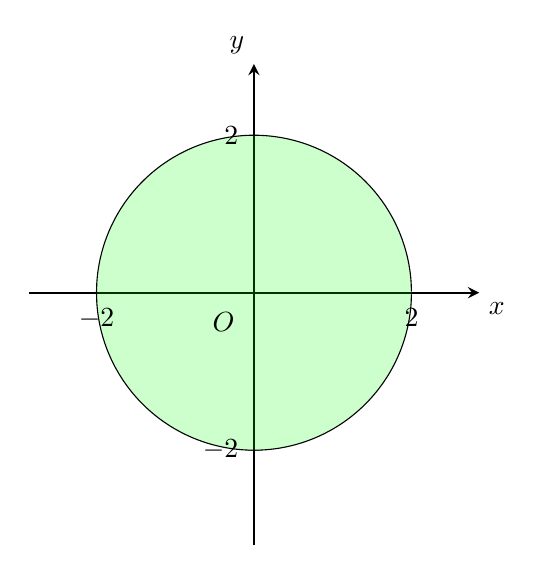
\begin{tikzpicture}
    \begin{axis}[standard,
            xtick={-2,2},
            ytick={-2,2},
            samples=1000,
            xlabel={$x$},
            ylabel={$y$},
            xmin=-2.2,xmax=2.2,
            ymin=-2.5,ymax=2.2,
            x=1cm,
            y=1cm/1
           ]
\node[anchor=center,label=south west:$O$] at (axis cs:0,0){};
\addplot[name path=F,domain={-2:2}]{sqrt(4-x^2)};
\addplot[name path=G,domain={-2:2}]{-sqrt(4-x^2)};
\addplot[fill=green, fill opacity=0.2] fill between [of=F and G,soft clip={domain=-2:2}];
    \end{axis}
    \end{tikzpicture}
}
\end{center}

Our lower and upper bounds for $r$ are $r=0$ and $r=2$, respectively.

Our lower and upper bounds for $\theta$ are $\theta=0$ and $\theta=2\pi$, respectively.

Putting this all together, we get
\begin{align*}
    V&=\int_0^{2\pi}\int_0^{2}\int_2^{\sqrt{8-r^2}}r\,dz\,dr\,d\theta\\
    &=\int_0^{2\pi}\int_0^{2}\lrb{rz}_2^{\sqrt{8-r^2}}\,dr\,d\theta\\
    &=\int_0^{2\pi}\int_0^{2} r\sqrt{8-r^2}-2r\,dr\,d\theta\\
    &=\int_0^{2\pi}\lrb{-\frac{1}{3}(8-r^2)^{3/2}-r^2}_0^2\,d\theta\\
    &=\int_0^{2\pi}\lrp{-\frac{1}{3}\lrp{8-4}^{3/2}-4}-\lrp{-\frac{1}{3}(8)^{3/2}-0}\,d\theta\\
    &=\int_0^{2\pi}\lrp{-\frac{8}{3}-4}+\frac{16}{3}\sqrt{2}\,d\theta\\
    &=\int_0^{2\pi}-\frac{20}{3}+\frac{16}{3}\sqrt{2}\,d\theta\\
    &=\lrb{-\frac{20}{3}\theta+\frac{16}{3}\sqrt{2}\theta}_0^{2\pi}\\
    &=-\frac{40}{3}\pi+\frac{32}{3}\sqrt{2}\pi\\
    &=\boxed{\lrp{\frac{-40+32\sqrt{2}}{3}}\pi}
\end{align*}
\phantomsection
\addcontentsline{toc}{subsection}{Spherical Coordinates}\textbf{Spherical Coordinates}

We can get our upper and lower bounds for $\rho$ from $x^2+y^2+z^2=8$ and $z=2$.

For our upper bound,
\begin{align*}
    x^2+y^2+z^2&=8\\
    \rho^2&=8\tag{$x^2+y^2+z^2=\rho^2$ in spherical}\\
    \rho &= \sqrt{8}\tag{keep positive only}
\end{align*}
For our lower bound,
\begin{align*}
    z&=2\\
    \rho \cos \phi &= 2\tag{$z=\rho\cos\phi$ in spherical}\\
    \rho &=  2\sec\phi
\end{align*}
We can get our upper and lower bounds for $\phi$ from the ``front view". Let's graph $\rho = \sqrt{8}$ and $z=2$.
\begin{center}
\resizebox{3.5cm}{!}{
    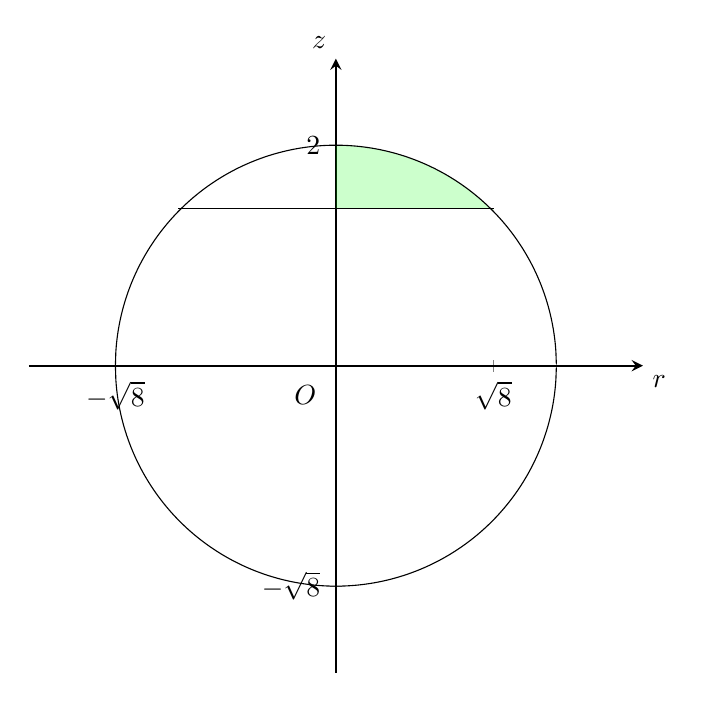
\begin{tikzpicture}
    \begin{axis}[standard,
            xtick={-2.8,2,2.8},
            ytick={-2.8,2.8},
            samples=1000,
            xlabel={$r$},
            ylabel={$z$},
            xmin=-3,xmax=3,
            ymin=-3,ymax=3,
            x=1cm,
            y=1cm/1,
            xticklabels={$-\sqrt{8}$, $\sqrt{8}$},
            yticklabels={$-\sqrt{8}$,$2$, $\sqrt{8}$}
           ]
\node[anchor=center,label=south west:$O$] at (axis cs:0,0){};
\addplot[name path=F,domain={-2.8:2.8}]{sqrt(2.8^2-x^2)};
\addplot[name path=G,domain={-2.8:2.8}]{-sqrt(2.8^2-x^2)};
\addplot[name path=H, domain={-2:2}]{2};
\addplot[fill=green, fill opacity=0.2] fill between [of=F and H,soft clip={domain=0:2}];
    \end{axis}
    \end{tikzpicture}
}
\end{center}
Our lower bound for $\phi$ is $\phi =0$.

We can get our upper bound of $\phi$ from the intersections of $z=2$ and $x^2+y^2+z^2=8\implies r^2+z^2=8$.
\begin{align*}
    r^2+z^2&=8\\
    r^2+2^2&=8\\
    r^2&=4\\
    r=2\\
    \phi &= \tan^{-1}\lrp{\frac{2}{2}}=\tan^{-1}(1)=\frac{\pi}{4}
\end{align*}
We're going around the entire $z$ axis for our ``top view" so our lower and upper bounds of $\theta$ are $\theta=0$ and $\theta=2\pi$, respectively. You can also verify this with the ``top view" (check our the Cylindrical Coordinates section for that).

Putting this all together, we get
\begin{align*}
    V&=\int_0^{2\pi}\int_0^{\pi/4}\int_{2\sec\phi}^{2\sqrt{2}}\rho^2\sin\phi \,d\rho\,d\phi\,d\theta\\
    &=\int_0^{2\pi}\int_0^{\pi/4}\lrb{\frac{1}{3}\rho^3\sin\phi}_{2\sec\phi}^{2\sqrt{2}}\,d\phi\,d\theta\\
    &=\int_0^{2\pi}\int_0^{\pi/4} \frac{16\sqrt{2}}{3}\sin\phi -\frac{8}{3}\sec^3\phi\sin\phi \,d\phi\,d\theta\\
    &=\int_0^{2\pi}\int_0^{\pi/4} \frac{16\sqrt{2}}{3}\sin\phi -\frac{8}{3}\tan\phi \sec^2\phi \,d\phi\,d\theta\tag{$\displaystyle \sec^3\phi\sin\phi =\sec^2\phi \frac{1}{\cos\phi}\sin\phi=\sec^2\phi\tan\phi$}\\
    &=\int_0^{2\pi}\lrb{-\frac{16\sqrt{2}}{3}\cos\phi-\frac{8}{6}\tan^2\phi}_0^{\pi/4}\,d\theta\\
    &=\int_0^{2\pi}\lrp{-\frac{16\sqrt{2}}{3}\lrp{\frac{1}{\sqrt{2}}}-\frac{8}{6}}-\lrp{-\frac{16\sqrt{2}}{3}-0}\,d\theta\\
    &=\int_0^{2\pi} -\frac{16}{3}-\frac{4}{3}+\frac{16\sqrt{2}}{3}\,d\theta\\
    &=\int_0^{2\pi}-\frac{20+16\sqrt{2}}{3}\,d\theta\\
&=\lrb{\frac{-20+16\sqrt{2}}{3}\theta}_0^{2\pi}\\
    &=\boxed{\lrp{\frac{-40+32\sqrt{2}}{3}}\pi}
\end{align*}
\phantomsection
\addcontentsline{toc}{section}{Problem 9}\textbf{Problem 9}

Find the centroid of the ``triangular" region bounded by the lines $x=2$ and $y=2$ and the hyperbola $xy=2$.

\Solution

For $M$,
\begin{align*}
    M&=\int_1^2\int_{2/x}^2\,dy\,dx\\
    &=\int_1^2\lrb{y}_{2/x}^2\,dx\\
    &=\int_1^2 2 -\frac{2}{x}\,dx\\
    &=\lrb{2x-2\ln\left|x\right|}_1^2\\
    &=\lrp{4-2\ln 2}-\lrp{2-2\ln 1}\\
    &={2-\ln 4}\tag{$2\ln2=\ln 2^2=\ln4$}
\end{align*}
For $M_{x}$,
\begin{align*}
    M_x&=\int_1^2\int_{2/x}^2 y\,dy\,dx\\
    &=\int_1^2\lrb{\frac{1}{2}y^2}_{2/x}^2\,dx\\
    &=\int_1^2 \frac{1}{2}(2)^2 - \frac{1}{2}\lrp{\frac{2}{x}}^2\,dx\\
    &=\int_1^2 2 - \frac{2}{x^2}\,dx\\
    &=\lrb{2x+\frac{2}{x}}_1^2\\
    &=\lrp{4+1}-\lrp{2+2}\\
    &={1}
\end{align*}
For $M_{y}$,
\begin{align*}
    M_y&=\int_1^2\int_{2/x}^2 x\,dy\,dx\\
    &=\int_1^2\lrb{xy}_{2/x}^2\,dx\\
    &=\int_1^2 2x - 2\,dx\\
    &=\lrb{x^2-2x}_1^2\\
    &=\lrp{4-4}-\lrp{1-2}\\
    &=1
\end{align*}
Our final answer is
\begin{subequations}
    \begin{empheq}[box=\widefbox]{align}
        \overline{x}&=\frac{M_{y}}{M}=\frac{1}{2-\ln 4}\nonumber\\
        \overline{y}&=\frac{M_{x}}{M}=\frac{1}{2-\ln 4}\nonumber\\
        \text{center of mass:}&
        \lrp{\frac{1}{2-\ln 4},\frac{1}{2-\ln 4}}\nonumber
    \end{empheq}
\end{subequations}
You could have also noticed that there's symmetry with respect to $y=x$, so $\overline{x}=\overline{y}$.
\newpage
\phantomsection
\addcontentsline{toc}{section}{Problem 10}
\textbf{Problem 10}

Use the substitution $u=x-y$, $v=y$ to show that
\begin{equation*}
    \int_0^\infty\int_0^xe^{-sx}f(x-y,y)\,dy\,dx=\int_0^\infty\int_0^\infty e^{-s(u+v)}f(u,v)\,du\,dv
\end{equation*}
if $f$ is any continuous function.

\Solution

\phantomsection
\addcontentsline{toc}{subsection}{Finding u, v, partials, and Jacobian}\textbf{Finding $u$, $v$, partials, and Jacobian}


We know that $y$ is in terms of $u$ and $v$. It's $y=v$. Let's use that knowledge in the equation $u=x-y$ by plugging in $y=v$ and solving for $x$.
\begin{align*}
   y&=v\\
   u&=x-v\\
   \implies x &= u+v
\end{align*}
Now, let's get our partials and Jacobian.
\begin{align*}
    \frac{\partial x}{\partial u}&= 1\\
   \frac{\partial x}{\partial v}&=1\\
   \frac{\partial y}{\partial u}&=0\\
   \frac{\partial y}{\partial v}&=1\\
    \begin{vmatrix}
    \frac{\partial x}{\partial u} & \frac{\partial x}{\partial v}\\
    \frac{\partial y}{\partial u} & 
    \frac{\partial y}{\partial v}
    \end{vmatrix}&=\begin{vmatrix}
      1 & 1\\
      0 & 1
    \end{vmatrix}=(1)(1)-(1)(0)=1
\end{align*}
\phantomsection
\addcontentsline{toc}{subsection}{Getting the uv region}\textbf{Getting the $uv$ region}

Let's translate our $xy$ region into a $uv$ region.

For $y=0$,
\begin{align*}
    y&=0\\
   \implies v&=0
\end{align*}
For $y=x$,
\begin{align*}
   y&=x\\
  \implies v&=u+v\\
   u&=0
\end{align*}
Our possible region ends up being one of the four quadrants. However, let's do some deductions to figure out which region is actually is.

We know that $y=v$. Since our $y$ values were always positive in the original region (graph $y=x$ when $x>0$), we know that our $v$ must always be positive as well. Therefore, our lower bound for $v$ is $0$ and our upper bound for $v$ is $\infty$.

Our lower bound for $u$ is $0$ and our upper bound for $u$ must be $\infty$.

\phantomsection
\addcontentsline{toc}{subsection}{Substituting In integral}\textbf{Substituting In integral}

We already know our region bounds. We also know $x=u+v$, $y=v$, and $x-y=(u+v)-v=u$.

Putting this all together, we get
\begin{align*}
    \int_0^\infty\int_0^xe^{-sx}f(x-y,y)\,dy\,dx=\int_0^\infty\int_0^\infty e^{-s(u+v)}f(u,v)\,du\,dv
\end{align*}
\end{document}
